\section{Results and Discussion}
\label{sec:midsurfcelljoin:results}
%
%The overall algorithm has been implemented as the following modules:
%\begin{enumerate}[noitemsep,topsep=2pt,parsep=2pt,partopsep=2pt]
%\item \textbf{Midcurve computation}: Uses a sketch profile in the form of a facetted polygon and generates a midcurve \cite{YogeshETES2014}.
%\item \textbf{Feature-based midsurface patch computation}: Computes the midsurface patch of a given cell-body using the owner feature parameters \cite{YogeshCOEP2013, YogeshIITG2014}.
%\item \textbf{Joining midsurface patches}: Uses the graph of cellular bodies and joins the midsurface patches at the interface cells.
%\end{enumerate}
%
%The first module is written in C\#, where as the others are implemented using the  Autodesk Inventor Application Programming Interface (API) in Visual Basic.Net. Following real-life part demonstrates the result  run on an Intel i3 64-bit 2 GHz Windows 7 machine:

This section demonstrates efficacy of the proposed midsurface computation approach, presented in this chapter, on a real-life part's CAD model. It is a commonly used sheet metal bracket. It consists of various features such as face, flange, holes etc. The model is assumed to be defeatured and generalized. 

\begin{itemize}[noitemsep,topsep=2pt,parsep=2pt,partopsep=2pt]
\item \textbf{Original Part}



\includegraphics[width=0.4\linewidth]{../Common/images/nonCellularBracket}

\item \textbf{Cellular Decomposition}

The original part has been decmposed into non-verlapping cells. $iCell$s are marked with dark-blue color whereas $sCells$ are shown in various colors.

\includegraphics[width=0.4\linewidth]{../Common/images/CellularBracket}

\item \textbf{Cellular Graph}

The cells are composed in the form of a cellular graph where nodes represent cells and edges represent connections.

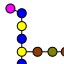
\includegraphics[width=0.3\linewidth]{../Common/images/CellGraphBracket.pdf}

\item \textbf{Midsurface}

The output shows computationn of well connected midsurface.

\includegraphics[width=0.4\linewidth]{../Common/images/midsCellularBracket}

\end{itemize}

%\section{Conclusion}
%\label{sec:midsurfcelljoin:conclusion}
%
%The proposed system transforms the complex feature tree of the model into a simplified one first, then  transforms them to generic Loft features. The model is decomposed into cells with owner-loft features. Feature parameters are leveraged to compute midsurface patches and a generic joining logic is used to connect the patches. The proposed methodology scores over existing approaches \cite{Chong2004, Cao2009, Cao2011, Woo2013, Boussuge2013, Boussuge2013a, Boussuge2014, Zhu2015} in terms of simplifying the complexities to a great extent and solving them rapidly.   It is not restricted by the underlying geometries as well as a few hard-coded connection types.
%
%%Feature generalization is used to compute the midsurface patches to address the face pair detection problem, whereas the feature based cellular decomposition  is used to address the midsurface patch interaction issues. This generic approach is advantageous as it is agnostic to underlying feature shapes as long as the basic methods of calculating the midsurface patches and joining are available for them.
%
%%Although individual functionalities such as defeaturing, abstraction and decomposition processes may show certain shortcomings, but overall, the proposed approach seems to work well and is able to compute a well-connected midsurface in robust, definitive and generic manner, with minimal failures.
%The algorithms were tested extensively on a wide range of academic as well as industrial sheet metal parts and it was observed that the mid surfaces were generated quite quickly and intuitively without any loss of connectivity within. There were a few pathological cases which the algorithms were not able to handle. However,  such corner cases were very limited and further advancements in the algorithms (not scoped in this work) can resolve these as well.
%
%
